\documentclass[aspectratio=169]{beamer}
\usetheme[
  block=fill,
  background=light,
  titleformat=smallcaps,
  progressbar=frametitle,
  numbering=none,
]{metropolis}
\usepackage{appendixnumberbeamer}
%%%%%%%%%%%%%%%%%%%%%%%%%%%%%%%%%%%%%%%%%%
%% Packages
%%%%%%%%%%%%%%%%%%%%%%%%%%%%%%%%%%%%%%%%%%

\usepackage{xspace} % no-argument aliases
\usepackage{amssymb}
\usepackage{amsmath}
\usepackage{cancel}
\usepackage{adjustbox}

% Colors
\usepackage{xcolor}
\usepackage{pifont}
\newcommand\greenCheck{\color{green!60!black}\ding{51}\xspace}
\newcommand\redCross{\color{red}\ding{55}\xspace}

% Tikz
\usepackage{tikz}
\usetikzlibrary{positioning,fit,calc,tikzmark,shapes.arrows,shapes.misc,arrows.meta}

% Images
\usepackage{graphics}
\graphicspath{{img/}}
\newcommand\agdaLogo{\raisebox{-1.5pt}{%

\includegraphics[keepaspectratio=true,height=2em,trim=0 5ex 0 0]{agda}}}

% Quotes
\usepackage{csquotes}
\SetBlockThreshold{2}
\newcommand\myblockquote[2]{%
  \blockquote{\hspace*{2em}\emph{`#1'}#2}\par}

% URLs as QR codes
\usepackage{qrcode}

% Agda
\usepackage{agda}
\setlength{\mathindent}{0em}
\AtBeginEnvironment{code}{\fontsize{9}{12}\selectfont}

\newcommand\agdaFont{JuliaMono}
\newcommand\agdaSerifFont{JuliaMono}
\newfontfamily{\AgdaSerifFont}{\agdaSerifFont}
\newfontfamily{\AgdaSansSerifFont}{\agdaFont}
\newfontfamily{\AgdaTypewriterFont}{\agdaFont}
\renewcommand{\AgdaFontStyle}[1]{{\AgdaSansSerifFont{}#1}}
\renewcommand{\AgdaKeywordFontStyle}[1]{{\AgdaSansSerifFont{}#1}}
\renewcommand{\AgdaStringFontStyle}[1]{{\AgdaTypewriterFont{}#1}}
\renewcommand{\AgdaCommentFontStyle}[1]{{\AgdaTypewriterFont{}#1}}
\renewcommand{\AgdaBoundFontStyle}[1]{\textit{\AgdaSerifFont{}#1}}

\newcommand{\AD}[1]{\AgdaDatatype{#1}}
\newcommand{\AC}[1]{\AgdaInductiveConstructor{#1}}
\newcommand{\AF}[1]{\AgdaFunction{#1}}
\newcommand{\AB}[1]{\AgdaBound{#1}}
\newcommand{\AK}[1]{\AgdaKeyword{#1}}
\newcommand{\AR}[1]{\AgdaField{#1}}

% vertical ellipsis between (visible parts of) code blocks
\newcommand\vdotsCode{\par{\hspace{1.5em}\raisebox{.3ex}{\(\smash\vdots\)}}\par}

%%%%%%%%%%%%%%%%%%%%%%%%%%%%%%%%%%%%%%%%%%
%% Fonts
%%%%%%%%%%%%%%%%%%%%%%%%%%%%%%%%%%%%%%%%%%
\usepackage{relsize}

% polytonic Greek in prose (same font as the website)
\newfontfamily\greekfont{GFS Didot}
\newcommand\gr[1]{{\greekfont #1}}
% single glyphs only JuliaMono has (ƛ, ϝ, ...)
\newcommand\jm[1]{{\AgdaSansSerifFont #1}}

%%%%%%%%%%%%%%%%%%%%%%%%%%%%%%%%%%%%%%%%%%
%% Macros
%%%%%%%%%%%%%%%%%%%%%%%%%%%%%%%%%%%%%%%%%%
\renewcommand\alert[1]{\textcolor{mLightBrown}{#1}}
\newcommand\todo[1]{\textcolor{red}{#1}}

% scansion marks in prose
\newcommand\qlong{\textbf{--}}
\newcommand\qshort{\raisebox{.35ex}{\smaller[2]\(\cup\)}}

% Pharr section references
\newcommand\pharr[1]{{\smaller\color{gray}[\S#1]}}


\newcommand{\blood}[1][1.5ex]{%
  \definecolor{bloodred}{RGB}{180,0,0}
  \adjustbox{valign=c}{%
    \begin{tikzpicture}[x=#1, y=#1, line join=round]
      % Main teardrop shape
      \fill[bloodred]
        (0, 1.1)
        .. controls (-0.1, 0.7) and (-0.6, 0.3) .. (-0.6, -0.1)
        arc (180:360:0.6)
        .. controls (0.6, 0.3) and (0.1, 0.7) .. (0, 1.1) -- cycle;
      % White specular glare highlight
      \fill[white, opacity=0.85]
        (0.2, 0.1) circle (0.1)
        (0.12, 0.32) circle (0.05);
    \end{tikzpicture}%
  }%
}
%----------------------------------------------------------------------------

\title{Formalising Homeric Prosody in Agda}

\author{\alert{Orestis Melkonian}, Konstantinos ``Kokos'' Kogkalidis}
\date{9 September 2026, Wadler70, Edinburgh}

\titlegraphic{%
\vspace*{4.5cm}\hfill
\parbox{3cm}{%
  \centering
  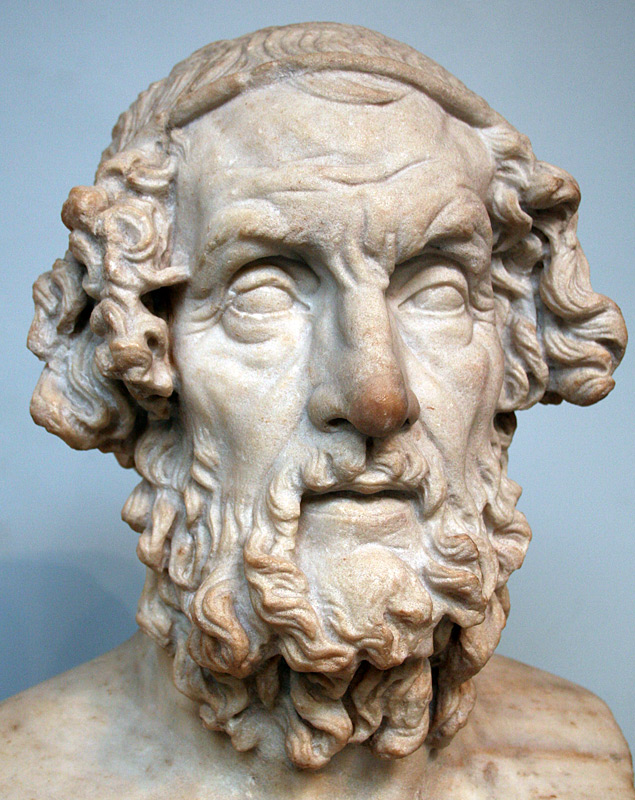
\includegraphics[keepaspectratio=true,height=2.5cm]{homer}\\[0.5em]
  \tiny{\emph{Marble portrait of Phil Wadler, British Museum}}
}
}

\newcommand\load[1]{\input{src/latex/#1}}

\begin{document}

% ** Agda setup
\AgdaNoSpaceAroundCode{}
\load{Morphology}
\load{Prosody}
\load{LevelOne}
\load{Flat}
\load{LevelTwo}
\load{LevelThree}
\load{Synizesis}
\load{LevelFour}
\load{Lexicon}
\load{Decidability}
\setbeamerfont{title}{size=\LARGE}
\setbeamerfont{subtitle}{size=\Large}

\begin{center}
\maketitle
\end{center}

%%%%%%%%%%%%%%%%%%%%%%%
%% INTRO
%%%%%%%%%%%%%%%%%%%%%%%

\begin{frame}{How it all started}
\begin{columns}
\begin{column}{.62\textwidth}
  \begin{itemize}
  \item Kokos approaches me with a \alert{challenge}:
  \begin{center}
  \emph{``let's formalise the rules of Homeric prosody''}
  \end{center}
  \vspace{1cm}
  \item<2-> always keen on such hobby-/side-projects
  \end{itemize}
  \vfill
  \onslide<2->{%
    \begin{center}
    \textbf{MOTTO:} \alert{breadth} \textbf{VS} depth
    \end{center}
  }
  \onslide<3->{%
    \begin{tikzpicture}[remember picture, overlay]
    \fbox{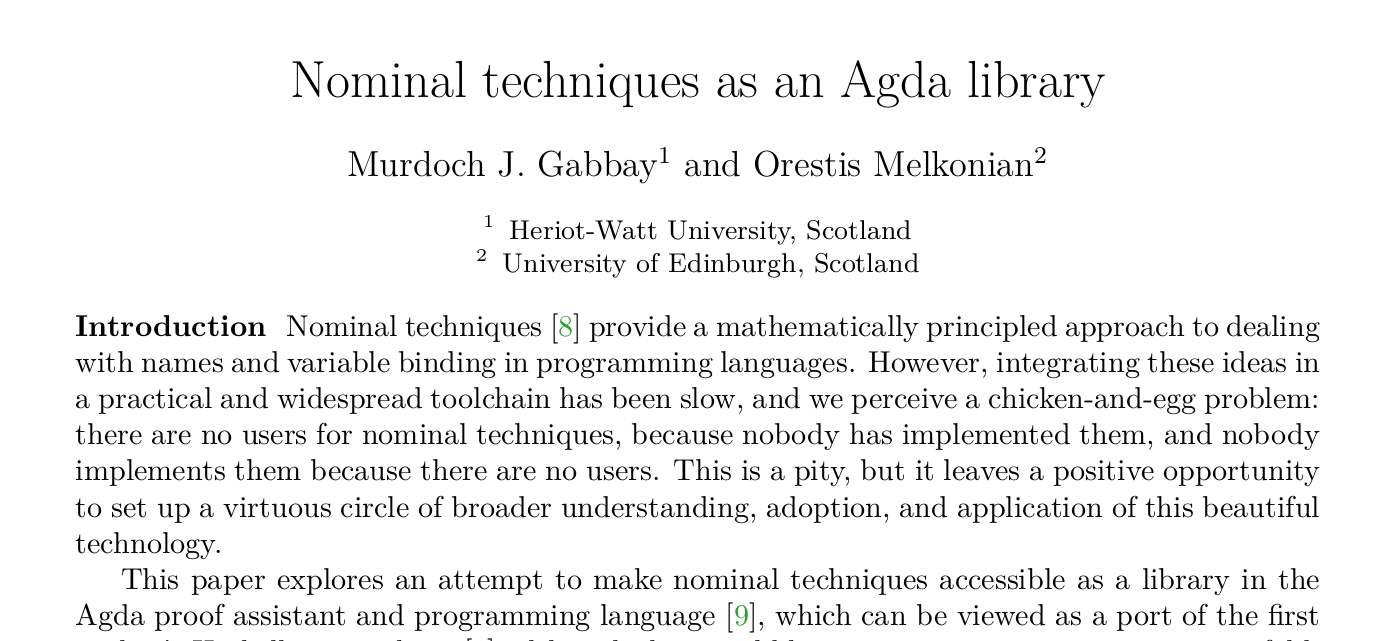
\includegraphics[keepaspectratio=true,height=3.5cm]{nom}}
    \end{tikzpicture}
  }
\end{column}
\begin{column}{.34\textwidth}
  \begin{center}
  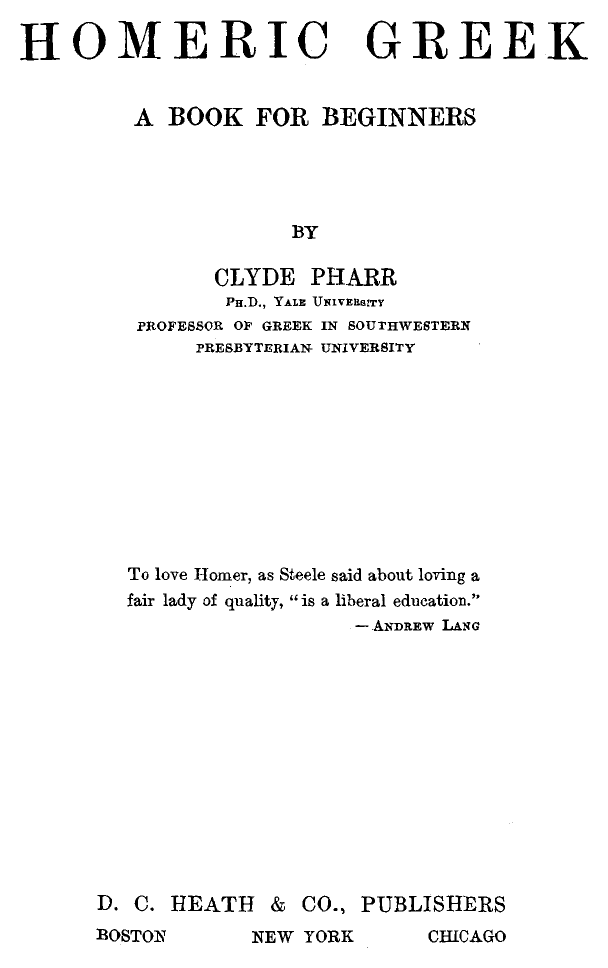
\includegraphics[keepaspectratio=true,height=.85\textheight]{pharr-cover}
  \end{center}
\end{column}
\end{columns}
\end{frame}

%%%%%%%%%%%%%%%%%%%%%%%
%% PROSODY CRASH COURSE
%%%%%%%%%%%%%%%%%%%%%%%

{\usebackgroundtemplate{%
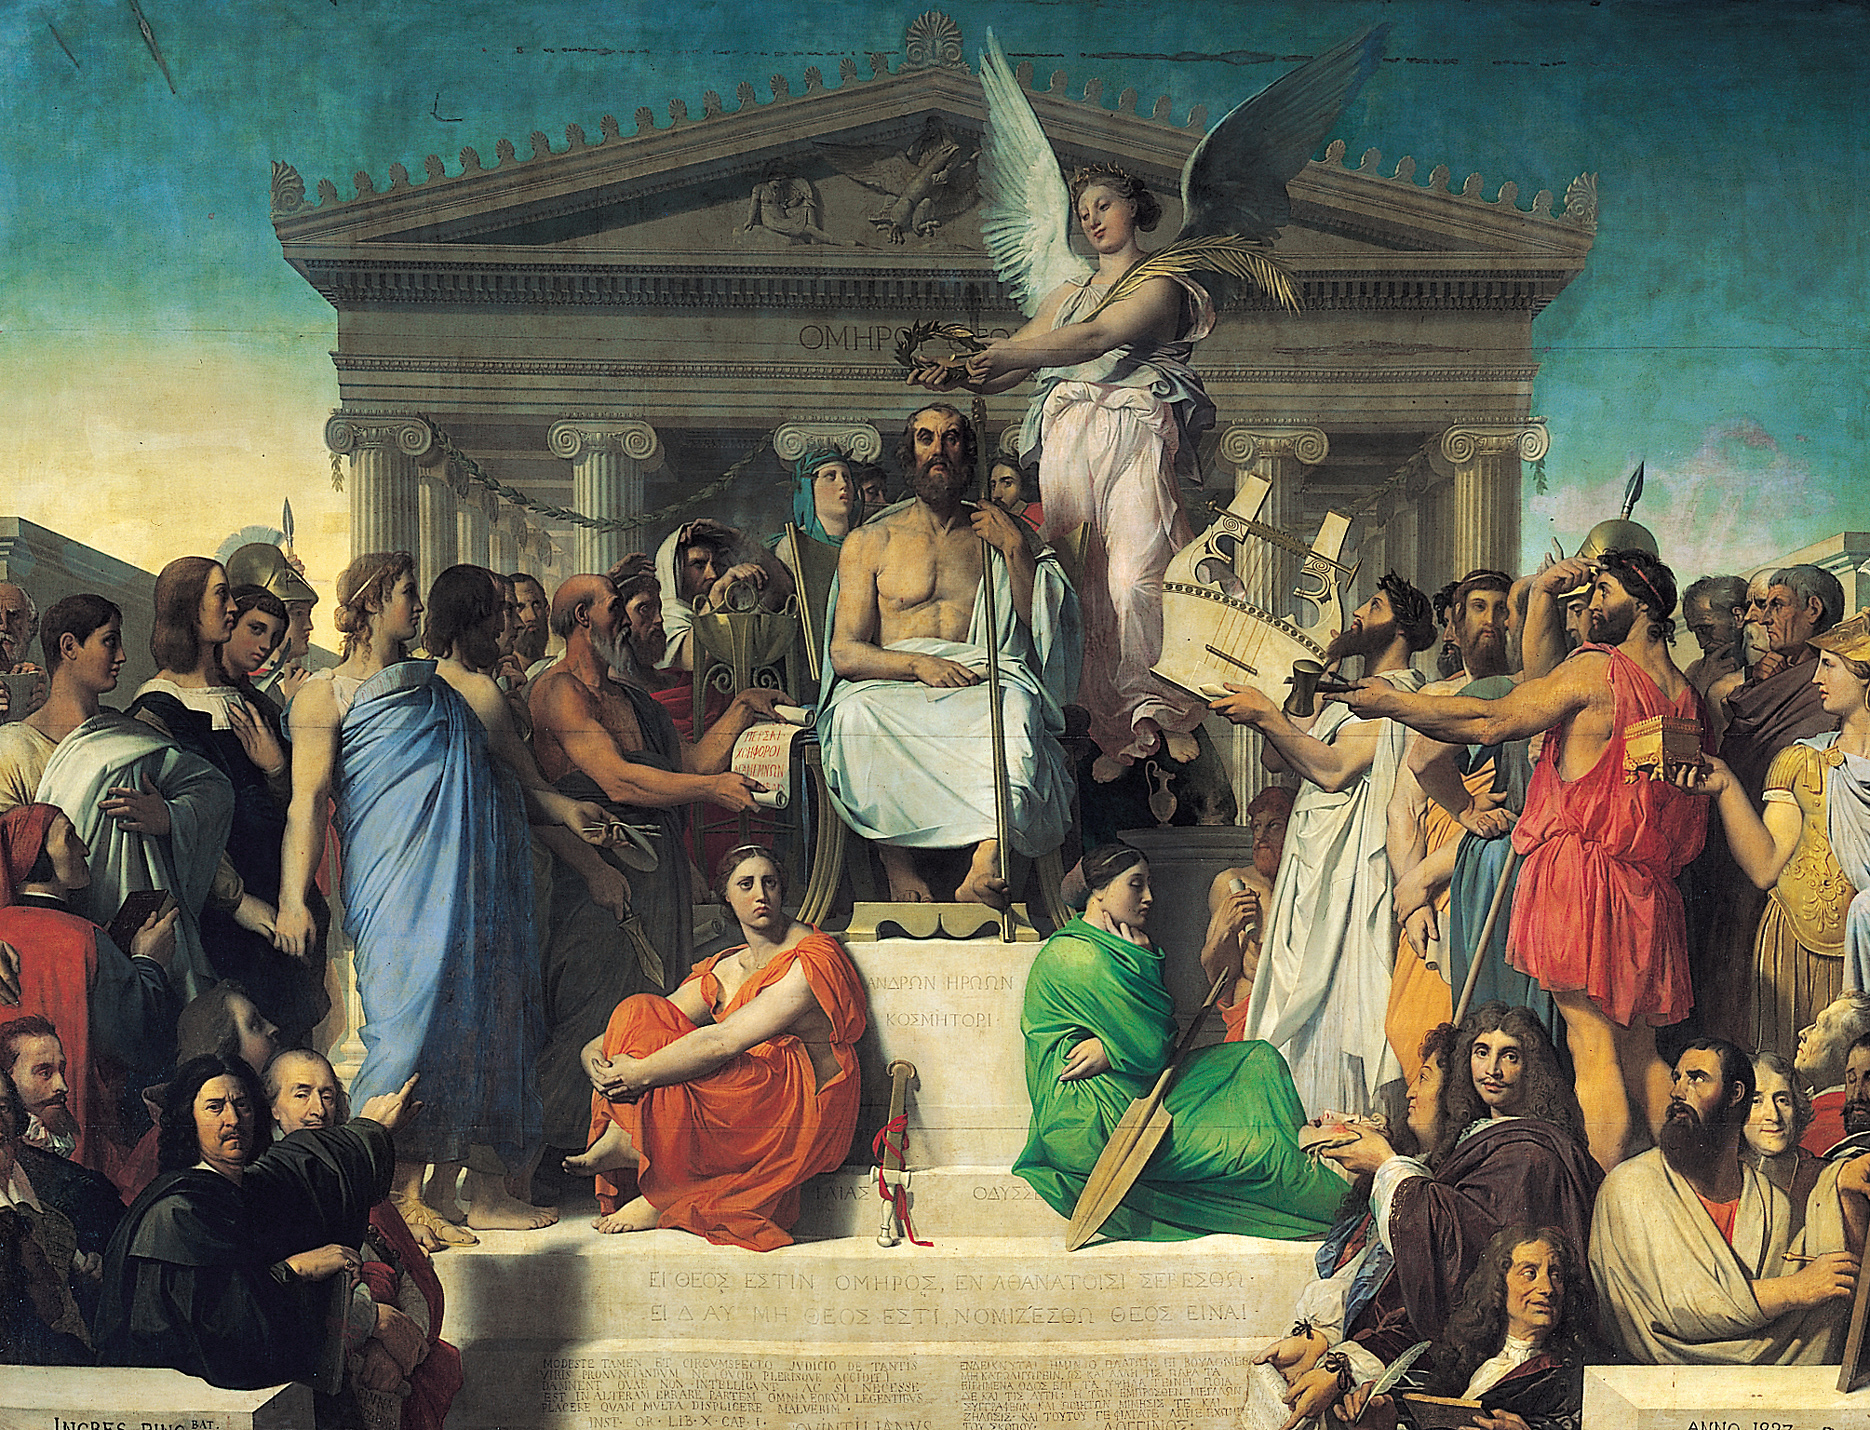
\includegraphics[width=\paperwidth]{ingres-homer}}
\begin{frame}{}\end{frame}}

\section{Prosody for the type theorist}

\begin{frame}{Prosody in one slide}
\begin{itemize}
\item a \alert{verse} is a sequence of \alert{syllables} (the Iliad has 15\,691 verses)
\item every syllable carries a \alert{quantity}: long (\qlong) or short (\qshort)
\item \alert{prosody} = the pattern of quantities a verse realises
\end{itemize}
\vfill
\begin{center}
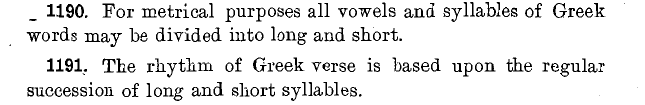
\includegraphics[width=.75\textwidth]{pharr-1190-1191}
\end{center}
\vfill
\pause
The very first verse of the Iliad:
\begin{center}
{\large
\begin{tabular}{*{16}{c}}
\qlong & \qshort & \qshort & \qlong & \qshort & \qshort & \qlong & \qlong &
\qlong & \qshort & \qshort & \qlong & \qshort & \qshort & \qlong & \qlong \\
\gr{μῆ} & \gr{νιν} & \gr{ἄ} & \gr{ει} & \gr{δε} & \gr{θε} & \gr{ὰ} & \gr{Πη} &
\gr{λη} & \gr{ϊ} & \gr{ά} & \gr{δεω} & \gr{Ἀ} & \gr{χι} & \gr{λῆ} & \gr{ος}
\end{tabular}}

\smallskip
{\small \emph{``Sing, goddess, the wrath of Achilles son of Peleus''}}
\end{center}
\end{frame}

\begin{frame}{Dactylic hexameter}
Homeric epics are written in \alert{dactylic hexameter}:
\begin{center}
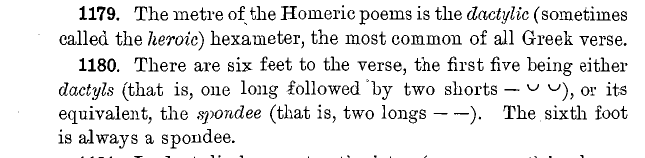
\includegraphics[width=.75\textwidth]{pharr-1179-1180}
\end{center}
\vfill
1 verse = 6 \alert{feet}, where foot = \alert{dactyl} (\qlong\,\qshort\,\qshort) or \alert{spondee} (\qlong\,\qlong):
\begin{center}
{\large
\begin{tabular}{ccc|ccc|cc|ccc|ccc|cc}
\qlong & \qshort & \qshort & \qlong & \qshort & \qshort & \qlong & \qlong &
\qlong & \qshort & \qshort & \qlong & \qshort & \qshort & \qlong & \qlong \\
\gr{μῆ} & \gr{νιν} & \gr{ἄ} & \gr{ει} & \gr{δε} & \gr{θε} & \gr{ὰ} & \gr{Πη} &
\gr{λη} & \gr{ϊ} & \gr{ά} & \gr{δεω} & \gr{Ἀ} & \gr{χι} & \gr{λῆ} & \gr{ος}
\end{tabular}}
\end{center}
\end{frame}

\begin{frame}{Scansion: the inverse problem}
\alert{Scansion} = inferring the meter from the written verse alone
\begin{itemize}
\item quantities are only \emph{partially} determined by spelling
\item the rest is constrained by accents, neighbouring syllables, \ldots\
      and \alert{the meter itself}
\end{itemize}
\vfill
\pause
\textbf{Existing tools are lacking in rigour:}
\begin{itemize}
\item automata \& ad-hoc systems in the digital humanities
\item the most popular site (\texttt{hypotactic.com}) provides scansion,
      but \alert{no explanations}
\item \alert{no resource that explains ALL of the Iliad}
\end{itemize}
\end{frame}

%%%%%%%%%%%%%%%%%%%%%%%
%% ILIAGDA
%%%%%%%%%%%%%%%%%%%%%%%

\section{Iliagda}

\begin{frame}{Reading Pharr: a constructivist's nightmare}
\only<1>{%
  \begin{center}
  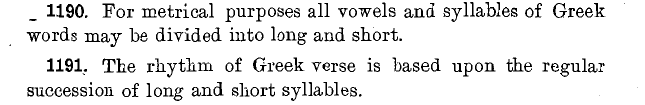
\includegraphics[width=.75\textwidth]{pharr-1190-1191}
  \end{center}
  \medskip
  \begin{itemize}
  \item unintuitive order: this is the \alert{last page!} of the book
  \item incoherent, conflating concerns, inconsistent naming
  \end{itemize}
}
\only<2>{%
  \begin{center}
  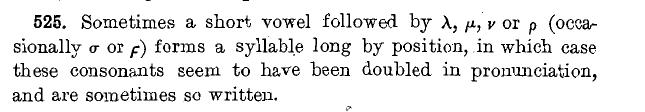
\includegraphics[width=.75\textwidth]{pharr-525}
  \end{center}
  \medskip
  \begin{itemize}
  \item too many \alert{modal} statements
  \end{itemize}
}
\only<3>{%
  \begin{center}
  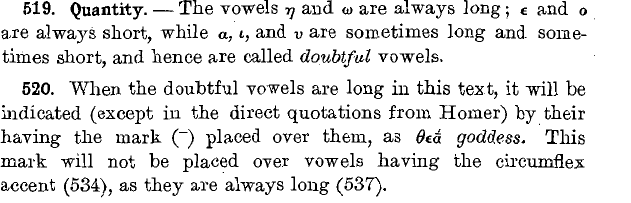
\includegraphics[width=.72\textwidth]{pharr-519-520}
  \end{center}
  \medskip
  quantities of \alert{doubtful} vowels are marked everywhere\ldots\
  \alert{except in Homer} (our input!)
}
\only<4>{%
  \begin{center}
  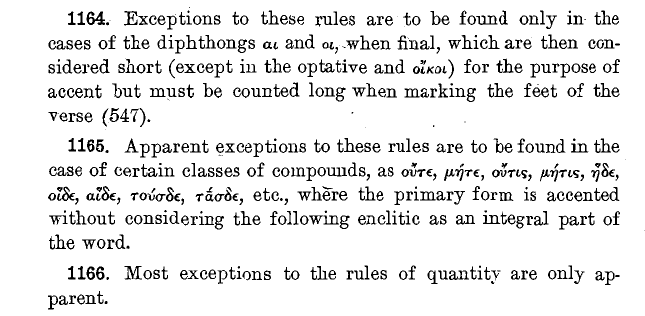
\includegraphics[width=.75\textwidth]{pharr-1164-1166}
  \end{center}
  \medskip
  \begin{itemize}
  \item exceptions, as well as ``apparent'' exceptions to the exceptions
  \item reminiscent of \alert{defeasible/default} logic, non-monotonic reasoning, etc.
  \end{itemize}
}
\only<5>{%
  \begin{center}
  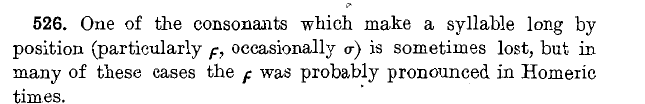
\includegraphics[width=.75\textwidth]{pharr-526}
  \end{center}
  \medskip
  \begin{itemize}
  \item \alert{lost} letters, despair\ldots
  \end{itemize}
}
\only<6>{%
  \begin{columns}[c]
  \begin{column}{.3\textwidth}
  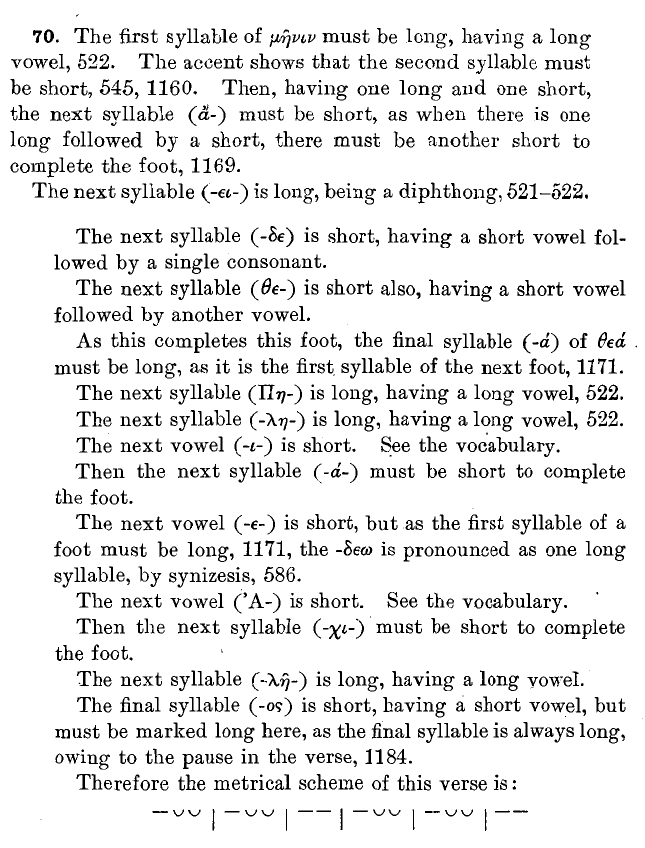
\includegraphics[keepaspectratio=true,height=.84\textheight]{pharr-70}
  \end{column}
  \begin{column}{.65\textwidth}
  \begin{itemize}
  \item \alert{few explanations}: just a single page out of \~400
  \end{itemize}
  \end{column}
  \end{columns}
}
\end{frame}

\begin{frame}{Architecture: declarative $\rightsquigarrow$ algorithmic}
Stratify the rules by \alert{how much context} they may consult:
\vfill
\begin{center}
\begin{tikzpicture}[
  lvl/.style={draw, rounded corners=2pt, align=center, minimum height=2.2em,
              inner sep=6pt, font=\small},
  lab/.style={font=\scriptsize\itshape, text=gray},
  arr/.style={-{Stealth[length=2mm]}, thick},
]
\node[lvl] (l1) {Level 1\\[-2pt]{\scriptsize syllable}\\[-1pt]
  {\tiny\color{gray}\gr{η ω} long, \gr{ε ο} short}};
\node[lvl, right=.7cm of l1] (l2) {Level 2\\[-2pt]{\scriptsize word/accents}\\[-1pt]
  {\tiny\color{gray}circumflex, acute}};
\node[lvl, right=.7cm of l2] (l3) {Level 3\\[-2pt]{\scriptsize next syllable}\\[-1pt]
  {\tiny\color{gray}long by position}};
\node[lvl, right=.7cm of l3] (l4) {Level 4\\[-2pt]{\scriptsize whole verse}\\[-1pt]
  {\tiny\color{gray}6 feet, final pause}};
\draw[arr] (l1) -- (l2);
\draw[arr] (l2) -- (l3);
\draw[arr] (l3) -- (l4);
\node[lvl, dashed, above=.6cm of l2] (lex) {\scriptsize Lexicon \& Readings};
\draw[arr, dashed] (lex) -- (l2);
\node[lvl, dashed] (syn) at ($(l2.south)!0.5!(l3.south)+(0,-1.1)$) {\scriptsize Synizesis [586]};
\draw[arr, dashed] (l2.south) |- (syn.west);
\draw[arr, dashed] (syn.east) -| (l3.south);
\end{tikzpicture}
\end{center}
\vfill
\pause
\begin{itemize}
\item each level emits \alert{partial knowledge} about quantities
\item Level 4 \alert{reifies}: only fully determined assignments form feet
\end{itemize}
\end{frame}

\begin{frame}{Morphology}
\only<1>{%
  \morphLetters
  \medskip
}
\only<2>{%
  \morphWords
  \medskip

  \begin{itemize}
  \item \textbf{words} indexed by their number of syllables
  \item a \textbf{verse} is just \AD{Words}~\AB{n}: concatenation tracks \AB{n} at the type level
  \end{itemize}
}
\end{frame}

\begin{frame}{Quantities \& meters}
\scalebox{.85}{\vbox{%
\prosodyQuantity
\medskip
\prosodyFoot
\medskip
\prosodyMeter
}}
\vfill
\begin{itemize}
\item \textbf{feet} are indexed by their quantities
\item \textbf{hexameters}: 6 feet over \AB{n} syllables
\end{itemize}
\end{frame}

\begin{frame}{Everything is a compliance relation}
\complies
\vfill
\begin{itemize}
\item one interface, instantiated at \alert{every} level:
  \begin{itemize}
  \item syllable\({}\sim{}\)quantity, word\({}\sim{}\)quantities, verse\({}\sim{}\)hexameter, \ldots
  \end{itemize}
\item \AF{NonDerivable}: constructive ``there exist no possible derivation''
\end{itemize}
\end{frame}

\begin{frame}{Level 1: inherent quantity}
\only<1>{\scalebox{.78}{\vbox{\prosodyVowels}}
\medskip

the constructive reading of \pharr{519}:
\alert{doubtful} = neither derivably long nor derivably short}
\only<2>{\scalebox{.85}{\vbox{\levelOne}}}
\end{frame}

\begin{frame}{Modal? Just three-valued works!}
\begin{columns}[t]
\begin{column}{.4\textwidth}
\scalebox{.85}{\vbox{\flatQ}}
\end{column}
\begin{column}{.58\textwidth}
\scalebox{.72}{\vbox{\flatCombine}}
\end{column}
\end{columns}
\vfill
\pause
\begin{itemize}
\item \AC{none} = no opinion, \AC{single} = certain, \AC{all} = \emph{ambivalent}
      (long \alert{and} short)
\item levels combine with the \alert{right-biased} \AF{\_⊗\_}:
      later, more informed levels win
\end{itemize}
\end{frame}


\begin{frame}{Level 1: inherent quantity}
\scalebox{.85}{\vbox{\levelOneFlat}}
\medskip

doubtful vowels leave the judgement \alert{partial}: on to the next level
\end{frame}

\begin{frame}{Level 2: accents constrain the last three syllables}
\scalebox{.72}{\vbox{\levelTwo}}
\end{frame}

\begin{frame}{Level 2: default logic via stratification}
\scalebox{.7}{\vbox{\levelTwoExc}}
\end{frame}

\begin{frame}[fragile]{Level 3: peeking at the next syllable}
\only<1>{%
  \levelThreeCtx
  \medskip

  the context may cross a \alert{word boundary} (\AC{outer}): quantity depends on \alert{verse} structure
}
\only<2>{%
  \scalebox{.7}{\vbox{\levelThree}}
}
\only<3>{%
  \scalebox{.7}{\vbox{\levelThreeQ}}
  \medskip

  three-valued verdicts: \AC{ambiguous}, \AC{ambivalent} (\alert{common} syllables), \AC{certain}
}
\end{frame}

\begin{frame}{Level 4: feet, at last}
\only<1,2>{\tikzmarknode{masks}{%
  \scalebox{.8}{\vbox{\levelFourReify}}
}}
\only<2>{%
  \begin{tikzpicture}[remember picture, overlay]
    \node[draw=red!70!black,line width=.5pt,fill=white,
          rounded corners=2pt,inner sep=4pt,xshift=-5cm,yshift=-3cm]
         (masksimg) at (current page.north east) {
      \clipbox{0pt 0pt 3cm 0pt}{\scalebox{.7}{\vbox{\levelFourMasks}}}
    };
    \coordinate (start) at ([xshift=-1.1cm, yshift=-.25cm] masks.center);
    \coordinate (end) at (masksimg.west);
    \draw[->,>=stealth,thick,red!70!black,shorten >=2pt,shorten <=2pt]
         (start) to[out=0, in=-180] (end);
  \end{tikzpicture}
}
\only<3>{\scalebox{.75}{\vbox{\levelFourFeet}}}
\only<4>{\scalebox{.75}{\vbox{\levelFourBend}}}
\end{frame}

\begin{frame}{The whole pipeline in one rule}
\scalebox{.76}{\vbox{\pipeline}}
\vfill
\begin{center}
read \({\blacktriangleright}\) lexicon \& accents \({\ggg}\) \tikzmarknode{syn}{synizesis}
\({\ggg}\) context \({\ggg}\) meter
\end{center}

\only<2>{%
  \begin{tikzpicture}[remember picture, overlay]
    \node[draw=red!70!black,line width=.5pt,fill=white,
          rounded corners=2pt,inner sep=4pt,xshift=-6cm,yshift=-5.5cm]
         (synimg) at (current page.north east) {
      \scalebox{.7}{\vbox{\synizesis}}
    };
    \draw[->,>=stealth,thick,red!70!black,shorten >=2pt,shorten <=2pt]
         (syn.north) to[out=90, in=-90] (synimg.south);
  \end{tikzpicture}
}
\end{frame}

{\setbeamercolor{background canvas}{bg=mDarkTeal}%
\begin{frame}{}
\begin{center}
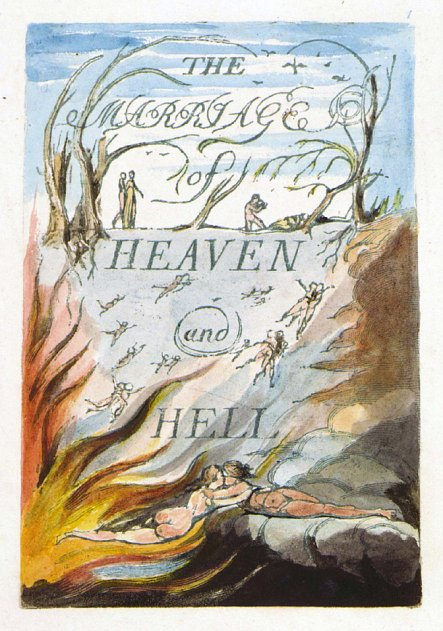
\includegraphics[keepaspectratio=true,height=\paperheight]{blake-mhh}
\end{center}
\end{frame}
}

\begin{frame}{The marriage of heaven \& hell: lexicon \& readings}
\begin{itemize}
\item pure rules meet reality: some quantities are just \alert{facts of the language}
\end{itemize}
\medskip

\begin{minipage}{.45\textwidth}
\scalebox{.7}{\vbox{\lexicon\vdotsCode}}
\end{minipage}
\hfill
\vrule
\hfill
\begin{minipage}{.5\textwidth}
\scalebox{.7}{\vbox{\reading\vdotsCode}}
\end{minipage}
\end{frame}

\begin{frame}{Decidability proofs as decision procedures}
\enumeration
\vfill\hrule\vfill
\allHexameters
\vfill
\pause
\begin{center}
scansion = \alert{running the spec};\quad
derivations then \alert{pretty-printed as explanations}
\end{center}
\end{frame}

\begin{frame}{Chasing the dragon}
\begin{itemize}
\item extracted to Haskell \& compiled; minor optimisations to keep proof search feasible
\end{itemize}
How many verses can we scan?
\begin{center}
{\Large 1 \quad\(\rightsquigarrow\)\quad \pause
10 \quad\(\rightsquigarrow\)\quad \pause
20 \quad\(\rightsquigarrow\)\quad \pause
50 \quad\(\rightsquigarrow\)\quad \pause
\alert{15\,679 / 15\,691} (>99.9\%)}
\end{center}
\vfill
\pause
\begin{itemize}
\item every new batch of verses \alert{falsified} our current reading of Pharr
\item corpus as the ground truth: rules were fixed, modified, re-stratified
\end{itemize}
\end{frame}

\begin{frame}{Epistemological BANG}
What about the remaining \alert{12} verses?
\medskip
\begin{itemize}
\item \alert{not logical gaps}: verses flagged as metrically anomalous in the literature
\pause
\item e.g.\ \alert{Δ 155}: {\large \gr{φίλε κασίγνητε θάνατόν νύ τοι ὅρκι᾽ ἔταμνον}} \\
      no consistent reading of Pharr's rules can scan it, \emph{``Homer was wrong''} :P
\pause
\item a formal system whose \alert{failures are philologically informative}
\pause
\begin{tikzpicture}[remember picture, overlay]
\hspace{-10cm}
\parbox{5cm}{%
  \centering
  
\includegraphics[keepaspectratio=true,height=2.5cm]{conor}\\[0.5em]
  \emph{Conor Titania Mc Bride}
}
\end{tikzpicture}
\end{itemize}
\end{frame}

\section{The website}

\begin{frame}{Every verse, explained, Hilbert style!}
\begin{center}
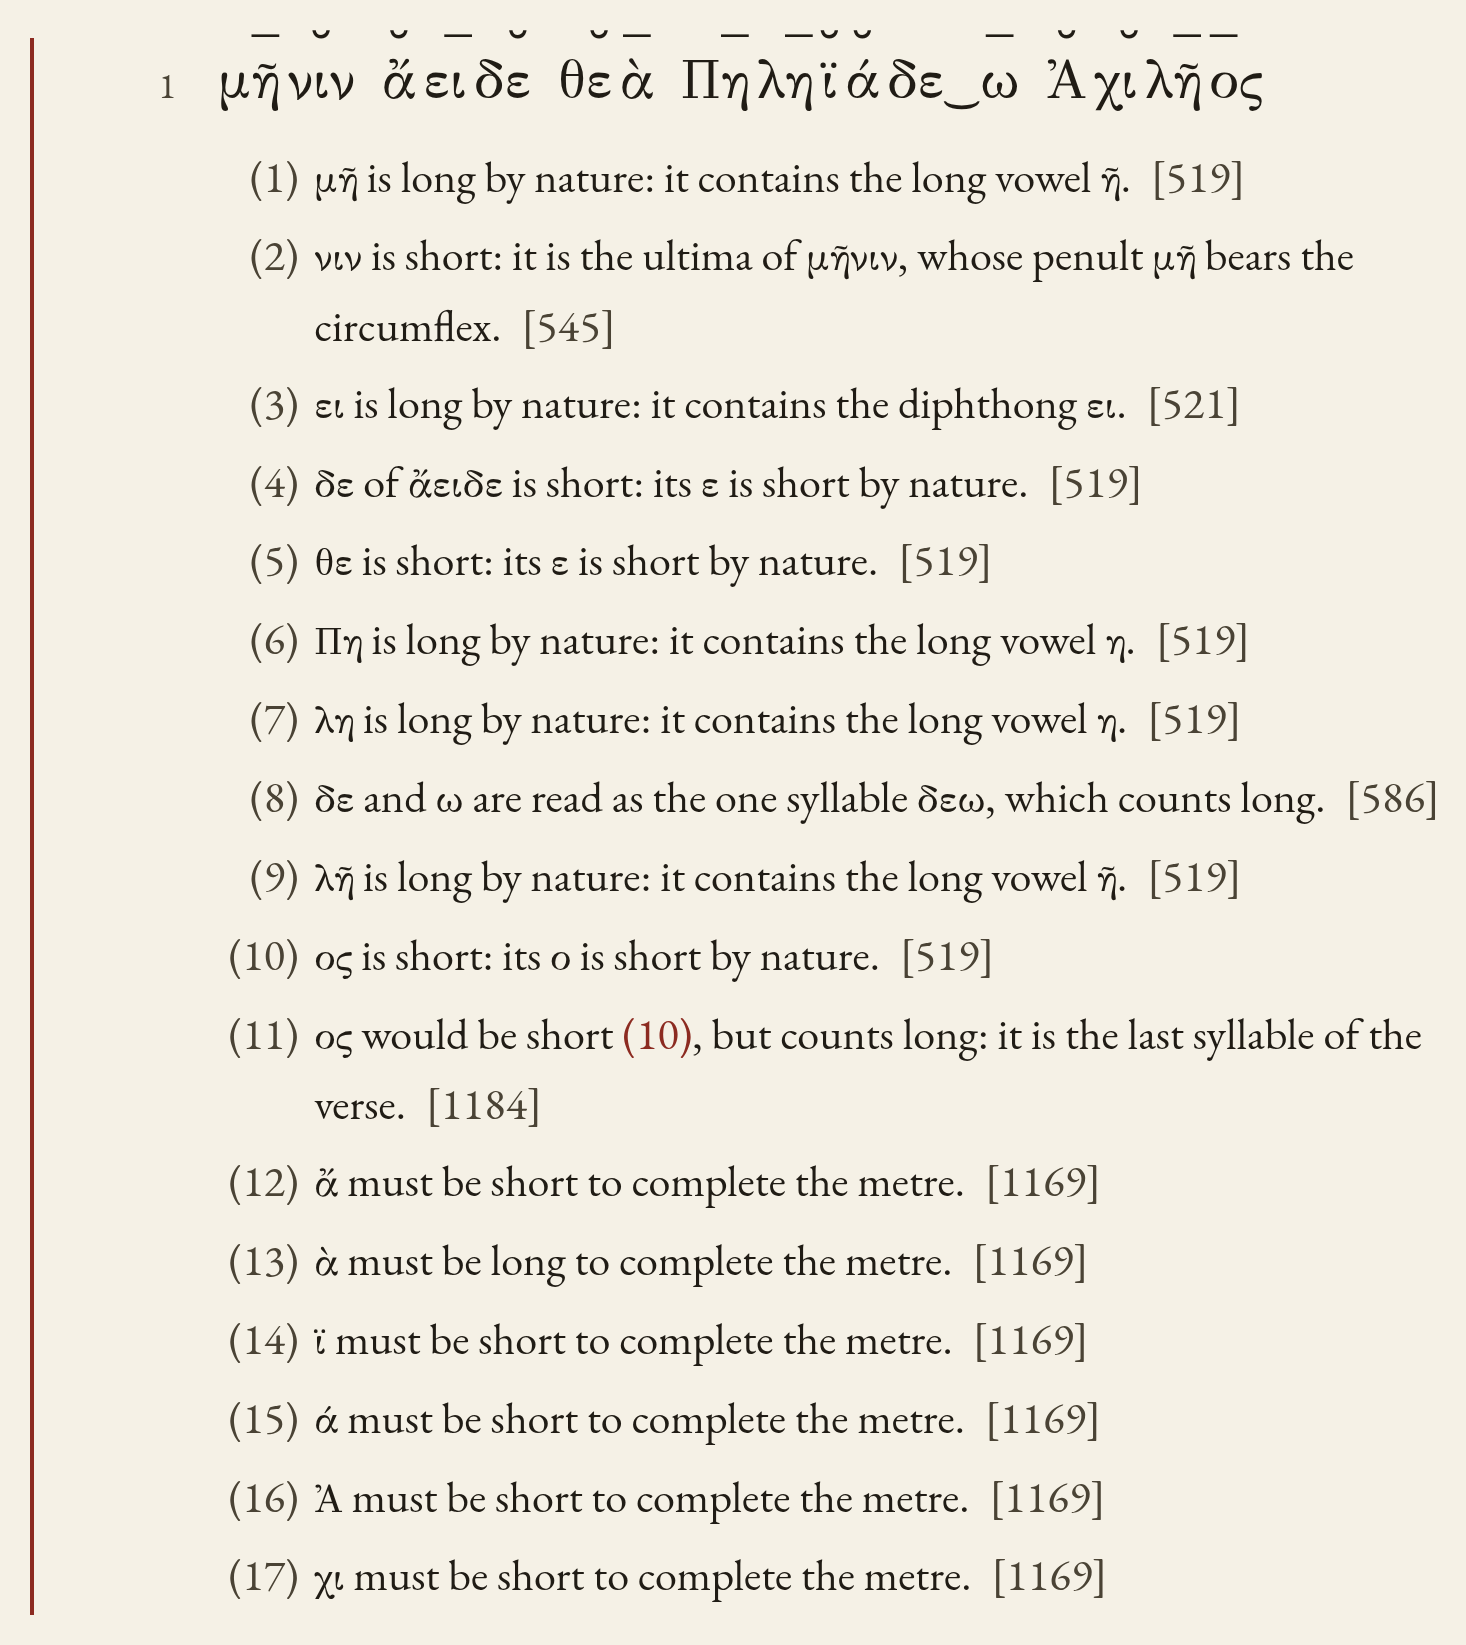
\includegraphics[keepaspectratio=true,height=.86\textheight]{site-v1}
\end{center}
\end{frame}

%%%%%%%%%%%%%%%%%%%%%%%
%% OUTRO
%%%%%%%%%%%%%%%%%%%%%%%

\begin{frame}{Conclusion}
We formalised Homeric prosody:
\begin{itemize}
\item Pharr's textbook as \alert{stratified inference rules}, mechanised in Agda;
\item \alert{sound \& complete} decision procedures = scansion with proofs;
\item already \alert{found faults} in \texttt{hypotactic.com} (e.g.\ Ι 382)
\item a website \alert{explaining (almost) every verse of the Iliad}, a first.
\end{itemize}
\pause
\textbf{Future work}
\begin{itemize}
\item other works: Odyssey, Ovid, \tikzmarknode{louis}{\textbf{Louis de G\'ongora (11-syllable)}}
\item beyond prosody: cover \alert{syllabification} as well
  \begin{itemize}
  \item towards a formal Ancient Greek grammar :O
  \end{itemize}
\item integrate into \alert{educational tools}
\end{itemize}
\pause
\begin{tikzpicture}[remember picture, overlay]
  %% \hspace{-10cm}
  \node[draw=red!70!black,line width=.5pt,fill=black, text=white,
        rounded corners=2pt,inner sep=4pt,xshift=-5cm,yshift=-2.3cm]
       (klapakisimg) at (current page.north east) {%
    \parbox{8cm}{%
      \centering
      \emph{\textbf{\tiny Shout-out to \alert{Michalis Klapakis}, my godfather and philologist extraordinaire!}}\\[.2cm]
      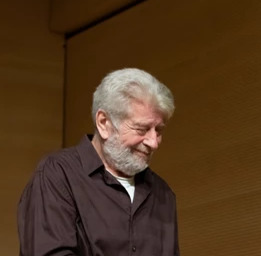
\includegraphics[keepaspectratio=true,height=3cm]{klapakis}
      \hspace{1cm}
      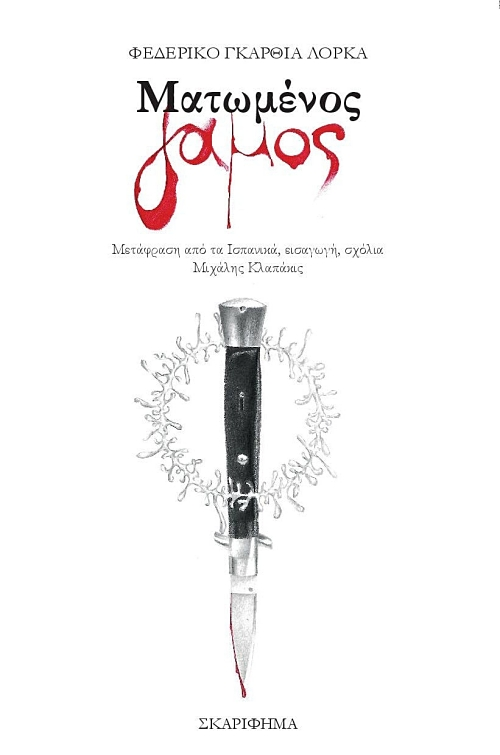
\includegraphics[keepaspectratio=true,height=3cm]{klapakis-lorca}
      %\\[0.5em]
    }
  };
  \coordinate (start) at ([xshift=-0cm, yshift=-0cm] louis.north);
  \coordinate (end) at (klapakisimg.south);
  \draw[->,>=stealth,thick,red!70!black,shorten >=2pt,shorten <=2pt]
       (start) to[out=90, in=-90] (end);
\end{tikzpicture}
\end{frame}

\begin{frame}{Reflection}

\textbf{Educational (for us)}
\begin{itemize}
\item a positivist who dodged Ancient Greek at school\ldots\
  \begin{itemize}
  \item \ldots now scans Homer \alert{by hand}, decently fast
  \item \emph{``\cancel{practice} rule-debugging makes perfect''}
  \end{itemize}
\end{itemize}

%% \vfill
\pause

\textbf{Educational (for others)}
\begin{itemize}
\item formalisation + website = study resource of \alert{unprecedented rigour}
\item every claim backed by a \alert{machine-checked derivation}
\end{itemize}

%% \vfill
\pause

\textbf{The Conquest of Bread(th)}
\begin{itemize}
\item push formal methods beyond math/software
\item towards Bogdanov's \emph{Proletkult}:
      organise all of science (\emph{tektology}) \ \blood
\end{itemize}

\end{frame}

\begin{frame}[standout]

{\Huge ¿¿¿ Questions ¿¿¿}
\vfill

\begin{center}
\qrcode[height=1in]{https://omelkonian.github.io/iliagda/}
\hfill
{\normalsize \alert{\url{https://omelkonian.github.io/iliagda/}}}
\end{center}
\end{frame}

\end{document}
